\chapter{Agents of Change}
\label{chap:agent}

According to Wikipedia today, Survivorship bias is the``logical error of concentrating on the people or things that made it past some selection process and overlooking those that did not, typically because of their lack of visibility. This can lead to false conclusions in several different ways. It is a form of selection bias'' \cite{wikipedia:survivorshipbias}. In other words, just because something happened ``against all odds,'' doesn't make it inevitable or a good idea. The problem is that those who tried something and failed often don't survive to tell the story and we end up hearing just from the unlikely survivors.

A great example of this is college drop-out entrepreneurs. I know the feeling of wanting to drop out because one has more pressing passions and projects, but I believe strongly that in most cases dropping out doesn't help people become successful, and others agree \cite{Zimmer:2013aa}. Any success that I've had is despite having dropped out of college and not because of it. I spent a lot of my time advising students to finish their degrees. :-)

In \autoref{sec:HAL} I wrote about our efforts to push computer science away from statistical correlations and towards causal relationships, asking if something we did actually caused the change or was it just something occurring at the same time. This relationship between outcomes through causal interventions is also the key to the theory of change described in \autoref{chap:theory} This is very difficult to derive without a randomized control study, but parts of my life have been quite random and I've tried some of my interventions over and over and in different ways, so I will try to sort out the generalizable causal interventions from the irrelevant ones. But as they say, ``Your mileage may vary.''

\section{Happiness}

In this dissertation, I have written at length about the goals of a system and the individuals in the system. The core aim of my thesis is to help shift the paradigm so that the goals of individuals and systems shift. My hope is that this will cause our systems to become more resilient, robust and sustainable.

The Declaration of Independence of the United States states that ``[A]ll men are created equal, that they are endowed by their Creator with certain unalienable Rights, that among these are Life, Liberty and the pursuit of Happiness.''

In ``The Art of Happiness'' the Dalai Lama also says that ``I believe that the very purpose of our life is to seek happiness.'' The Dalai Lama argues that happiness is more determined by the state of our minds than by our external conditions once our basic survival conditions have been met \cite{lama2009art}.

Abraham Maslow in his 1943 paper ``A Theory of Human Motivation'' argues that there are stages of growth in humans needs. He used the terms ``physiological'', ``safety,'' ``belonging and love,'' ``esteem,'' ``self-actualization,'' and ``self-transcendence'' to describe the layers in his ``hierarchy'' of needs pyramid\cite{maslow_theory_1943}. (See \autoref{fig:maslowpyramid}.) The lower layers of Maslow's hierarchy are fairly straight forward, but as one ascends to the higher layers such as social belonging, esteem, self-actualization and self-transcendence, the extrinsic versus intrinsic nature of the happiness or need is unclear. Self-transcendence was added by Maslow in his later years as he critically explored the dimension of needs beyond self-actualization.\ \cite{maslow1991critique}.

\begin{figure}[t]
 \centering
 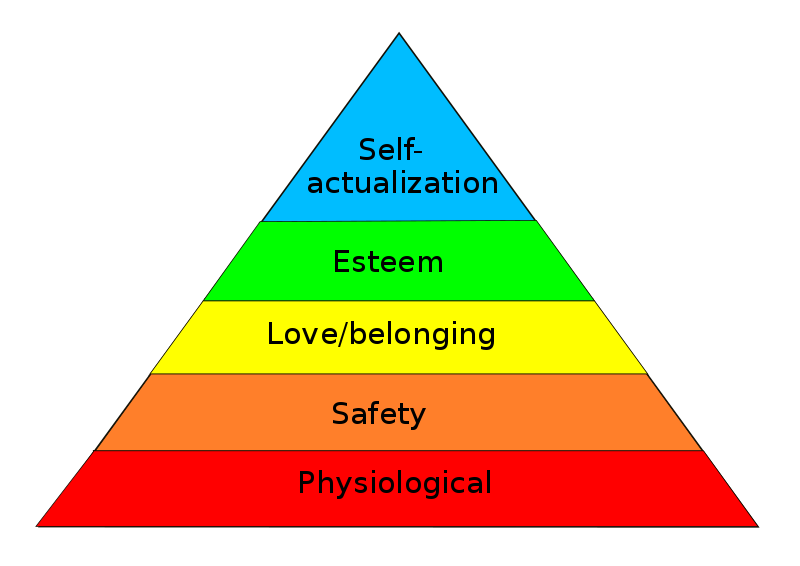
\includegraphics[width=.5\textwidth]{pictures/MaslowsHierarchyOfNeeds}
 \caption[Maslow's hierarchy of needs]{Maslow's hierarchy of needs, represented as a pyramid with the more basic needs at the bottom. Source: FireflySixtySeven via Wikipedia. \ccbysa}
 \label{fig:maslowpyramid}
\end{figure}

For example, esteem is mostly associated with extrinsic validation such as respect and recognition. However, self-esteem can be quite internal or intrinsic. Self-actualization includes art and athletics, which also have extrinsic and intrinsic motivations. Self-transcendence becomes less ego-oriented, but also can have motivations such as the need to help other humans, or intrinsic motivations such as becoming one with nature. It is clear that the higher levels of Maslow's hierarchy are less zero-sum and less competitive: the extrinsic versus intrinsic distinction changes the nature of the relationship between the individual and the community/society, as well as one's need to adhere to the social systems required for validation.

The Dalai Lama and the contemplative tradition focuses more on intrinsic motivations. While most contemplative traditions aren't necessarily anti-social, a diminished need for external validation for happiness lets one be less concerned with the opinions of others, providing more freedom and time to become self-aware and achieve happiness through the pursuit of one's personal passion or interests. This is an approach that The Venerable Tenzin Priyadarshi and I teach in my Principles of Awareness class described in \autoref{section:awareness}.

The Dalai Lama in \emph{The Art of Happiness} discusses the difference between pleasure and happiness and argues that many people feel ``happy'' when they get more money, get a new car, or progress along an externally provided measurable path. He defines these feelings as pleasures and suggests that the happiness that he describes is more like the happiness of having a happy family. Increasing the size of the family doesn't make one more happy. The Buddhist notion of happiness is quite different from happiness as described by economists who describe it as an increase in utility --- an economic measure \cite{marshall1961principles}. Later, utility was quantified by Paul Samuelson as ``revealed preference'' \cite{samuelson1948consumption} and apparently the more utility the better. The Buddhists would feel more aligned with the adage, ``more than enough is too much'' than the notion of the utility function.

\marginpar{I would suggest the word ``flourishing'' as a way to define happiness or goodness without a need to include progress or growth. A vibrant rainforest is a great example of a flourishing system.}However, many argue that progress is essential and without extrinsic motivations and economically rational humans, we would not have progress. For example, Matt Ridley argues in \emph{The Rational Optimist} that humans have an innate tendency or desire to trade. He argues that markets enable this exchange and that this exchange allows specialization --- I can help build the Internet that you use and you can design the motor for my car and use the Internet. He says that this market-based exchange of goods, services, ideas and products allows progress, and enables ideas to ``have sex'' --- computers and telecommunications coming together to turn into the Internet \cite{ridley_rational_2010}.

While the idea is exciting and helps describe how much of innovation works, he's also describing the system that, in my view, causes income inequality, exploitation of the environment, and the deployment of technologies of convenience at the cost of health. Indeed, he doesn't question whether progress is in fact ``good.''

I would suggest the word ``flourishing'' as a way to define happiness or goodness without a need to include progress or growth. A vibrant rainforest is a great example of a flourishing system. It doesn't need to grow in total size. There is diversity, there is growth and death together. There are many systems that are interconnected and the system is highly robust. While there is some controversy about methods, there is a scientific approach to measuring ecosystem robustness \cite{mumby2014ecological}. There is evolution and ``progress'' but it is slow and more like a slow adaptive search than the geometric growth or even exponential growth of human civilization.

This notion of flourishing is described in \autoref{sec:cultureflourish} and is what I believe that we must strive for in order to achieve sustainable and long-term resilience in our systems.

In \emph{The Human Use of Human Beings}, Norbert Wiener questions our idea that progress is necessarily good.

\begin{quotation}Those who uphold the idea of progress as an ethical principle regard this unlimited and quasi-spontaneous process of change as a Good Thing, and as the basis on which they guarantee to future generations a Heaven on Earth. It is possible to believe in progress as a fact without believing in progress as an ethical principle; but in the catechism of many Americans, the one goes with the other.\end{quotation}

As I wrote in the introduction, ``eudaimonia'' and productive self-actualization described by Aristotle in ``Nicomachaen Ethics`` \cite{rowe2002nicomachean} are useful concepts that includes the notions of progress towards ethics and flourishing.

\section{Interest-Driven Learning}

As I was saying, I dropped out of college twice and was even kicked out of kindergarten for running away too many times. I was never very good at education, but I liked to learn. One of my principles (see \autoref{principles}) is ``learning over education.'' I believe that education is what other people do to you and learning is what you do for yourself.

It wasn't that my schools were particularly bad or that I wasn't provided an opportunity. My sister got straight A's and went to Harvard and Stanford and got two Ph.D.s. I just had a personality that made it difficult for me to learn in a structured way about things that I didn't find useful or interesting. I also had a difficult time studying abstractions in books. I much preferred learning through doing things and talking to people.

It was very lucky for me that I was surrounded by scientists, nature, and then online computer networks and the Internet as I was entering high school. I was able to kludge together an understanding of the world's conversations by pursuing a wide variety of interests including working in a pet shop, being a disk jockey in a nightclub, working as an associate to the producer in a Hollywood film, working in a material science lab writing software for the control system, running an events company, running a computer peripherals mail order company, being a professional scuba instructor, being a record distributor, a columnist in a newspaper, a software distributor, an apparel distributor and many other things.

While I believe that I am unusually poor at structured learning, unusually motivated by my passions and interests, and unusually interested in almost everything, I do believe that interest-driven learning is generalizable.

In 1973, Ivan Illich wrote \emph{Tools for Conviviality} and argued that there are two pivotal moments in the history of scientific and societal progress. The first was in 1913 when Western medicine improved to the point where trained doctors could increase their patients odds past 50/50. The second was when we focused more on keeping people alive than on worrying about the quality of the patient's life or their agency. Illich writes, ``I choose the term `conviviality' to designate the opposite of industrial productivity. I intend it to mean autonomous and creative intercourse among persons, and the intercourse of persons with their environment; and this in contrast with the conditioned response of persons to the demands made upon them by others, and by a man-made environment'' \cite{Illich:1973aa}.

Illich blames professional elites and economic development for negatively impacting human flourishing in modern times by institutionalizing specialization and taking control of the tools of society away from the average citizen. He believes we must ``give people tools that guarantee their right to work with independent efficiency.''

This ties to his argument that modern education focuses on institutionalization and that, as he argues in 1971's \emph{Deschooling Society}, these institutions are reducing flourishing. He argues that the educational ``funnels'' must be reversed and that we must create ``learning webs'' using advanced technology \cite{Illich:1971aa}.

The Montessori Method \cite{montessori2013montessori} of child-centered education has been used for over 100 years \cite{montessoriintro}. While the Montessori Method is much more flexible and child-guided than traditional educational systems, it still provides a teacher who guides the child by observing and responding to the child's behavior and tendencies. Unschooling, which was coined in the 1970s by John Holt \cite{unschooling}, advocates an even more radical child-directed learning approach that focuses on freeing the child from any form of formal education, depending instead on our natural ability to learn, and a belief that we will learn what we need to learn in the course of doing what we are passionate about.

In my own experience, the only practical thing that I learned how to do in my secondary formal education was touch typing. Otherwise, everything I learned, I learned out of class, except perhaps social skills that I could easily learn through group activities rather than through by sitting in a classroom. As I consider the future of schooling for my one year old daughter, I am thinking deeply about different educational options.

Jean Piaget in the 1930s said that cognitive development in children occurs as children interact with the world around them. \cite{piaget1952origins}. Seymour Papert worked with Paiget at the University of Geneva from 1958 to 1963 \cite{SeymourP62:online} and was one of Piaget's protégés. Papert was a founding member of the MIT Media Lab and developed a theory of learning called Constructionism --- student-centered project-based learning-through-doing -- that is at the core of the Media Lab, as I described in \autoref{antidisciplinaryapproach}. Papert inspired others at the Media Lab including Mitchel Resnick who argues for cultivating creative learning through ``projects, passion, peers and play'' \cite{resnick_lifelong_2018}. Resnick developed the Scratch programming language to empower children to ``code to learn'' instead of ``learning to code.'' Neil Gershenfeld is a former Media Lab professor, the director for the Center for Bits and Atoms and the inventor of the Fab Lab (short for fabrication laboratory) and the creator of the Fab Academy, a learning network. He is trying to create a network of Fab Labs to bring learning-through-making to the rest of the world. Gershenfeld says that Fab also means fabulous --- a kind of flourishing that Illich would have approved of \cite{gershenfeld2008fab}.

I believe that creativity and passion will become even more important in the future and that jobs will become even more differentiated. I also believe that learning how to follow your personal passions, rather than depending on institutions to provide motivation, will be increasingly important as jobs change and institutions go through the current industrial transformation.

Passion can come from a variety of sources. In \emph{The Wealth of Networks}, Yochai Benkler explains that the motivations for many of the online communities to produce is not financial \cite{benkler2006wealth}. In \emph{Not Just for the Money} economist Bruno Frey argues that offering higher pay may make people less committed to their work and may reduce performance \cite{frey1997not}. The social context and our desire to collaborate is a key element in developing passions.

As I write in \autoref{intro:communityvalues} Nowak and Highfield describe the evolution of cooperation and mechanisms for cooperation. They argue that evolution is not only competition but also cooperation, and that cooperation is the master architect of complexity. In ``Spontaneous giving and calculated greed,'' researchers argue that people are intuitively cooperative and thus need to``calculate'' to overcome their cooperative impulse and become greedy \cite{rand2012spontaneous}. In ``Cooperating with the future'' \cite{hauser2014cooperating} the argument is that a large altruistic, majority would vote to cooperate with a longer view of the future in a democratic setting.

\section{Competition and Greed}

I also have competitive and greedy feelings sometimes, but they are fundamentally overpowered by my passion for the missions of my projects and my desire to collaborate and cooperate, which is supported by the studies above.

The following is an exchange on television between Phil Donahue and economist Milton Friedman from 1979 \cite{noauthor_notable_2015}:

\begin{quote}
Phil Donahue: When you see around the globe the maldistribution of wealth, the desperate plight of millions of people in underdeveloped countries, when you see so few haves and so many have-nots, when you see the greed and the concentration of power, did you ever have a moment of doubt about capitalism and whether greed’s a good idea to run on?

\marginpar{Milton Friedman: Well, first of all, tell me, is there some society you know that doesn’t run on greed? You think Russia doesn’t run on greed? You think China doesn’t run on greed? What is greed?}Milton Friedman: Well, first of all, tell me, is there some society you know that doesn’t run on greed? You think Russia doesn’t run on greed? You think China doesn’t run on greed? What is greed? Of course none of us are greedy. It’s only the other fellow who’s greedy. The world runs on individuals pursuing their separate interests. The great achievements of civilization have not come from government bureaus. Einstein didn’t construct his theory under order from a bureaucrat. Henry Ford didn’t revolutionize the automobile industry that way. In the only cases in which the masses have escaped from the kind of grinding poverty you’re talking about, the only cases in recorded history are where they have had capitalism and largely free trade. If you want to know where the masses are worst off, it’s exactly in the kinds of societies that depart from that. So that the record of history is absolutely crystal clear that there is no alternative way, so far discovered, of improving the lot of the ordinary people that can hold a candle to the productive activities that are unleashed by a free enterprise system.

Donahue: But it seems to reward not virtue as much as ability to manipulate the system.

Friedman: And what does reward virtue? . . . I think you’re taking a lot of things for granted. Just tell me where in the world you find these angels who are going to organize society for us.
\end{quote}

I think this exchange captures the essence of the capitalist ``greed is good'' philosophy that has caused the reductionist single-minded pursuit of personal wealth that has undermined robustness, resilience, flourishing and has crowded out many of the intrinsic and more positive extrinsic motivators in our society.

There is a place for competition and there is a role for self-interest, but these elements should be part of a complex system of values and drivers, and tend to address the lower elements of Maslow's hierarchy.

And one of the problems with Maslow's hierarchy is that it assumes we are individuals first and foremost. When it comes to how we run our academic system, why do we demand academics prove themselves as individuals rather than participants in a group. The tenure process and even the doctoral process focus on the individual even thought their work will almost inevitably occur within and because of a social web. Some fields, such as high energy experimental physics, have begun to be more open to large collective projects, but for the most part, academics are judged as individuals. In fact, this doctoral process required me to justify why I didn't have two single authored books and two single authored papers.

The tenure process as I have observed it at MIT has the same problem and pushes junior faculty to worry constantly about seeking external validation of their individual work.

I find that my staff, including my research staff, are fundamentally less competitive and more mission-oriented than the majority of the faculty at MIT. Yet their productivity and creativity exceeds all expectations. My impression is that they are happier as well.

I often wonder whether we can have the creativity and the drive required to make brilliant contributions to society without the competition that drives many of the significant achievements.

My experience with the leaders and the community members of Creative Commons and  Internet technical communities involved dealing with some level of ``drama'' --- competition, egos and greed --- but these people and incidents felt more like anomalies and ``problems'' than the normal behavior that Milton Friedman describes so well and is so institutionalized in traditional corporate environments and in some elements of academia.

Startups have a fair share of greed but many of the successful companies are able to also have a healthy cooperative and mission-oriented socially sensitive cultures as well. This could be a shift in the demographic as young people are more concerned about the systems and less driven by the greed of their neo-liberal economic parents. The 2016 Cone Communications Millennial Employee Engagement Study showed that 64 percent of Millennials in the US ``won’t take a job if a company doesn’t have strong corporate social responsibility (CSR) values'' \cite{conestudy}.

\section{Disobedience}

\marginpar{Martin Luther King Jr. wrote, “One has not only a legal but a moral responsibility to obey just laws. Conversely, one has a moral responsibility to disobey unjust laws'' \cite{king2012letter}.}Enjoying cooperation and flourishing does not mean that we must be obedient. For systems to evolve, they require variation, mutations and diversity. Disobedience is necessary to question the status quo in science, society, law or the arts. Timothy Leary used to tell me, ``Question authority and think for yourself.'' Martin Luther King Jr. wrote, “One has not only a legal but a moral responsibility to obey just laws. Conversely, one has a moral responsibility to disobey unjust laws'' \cite{king2012letter}.

A healthy democracy, a healthy academic institution, a healthy community must be disobedience-robust. In other words, people should be allowed and encouraged to speak up against those in power without fear of retribution, and the questioning should make the system more robust, not fragile. This requires a great deal of trust between the individuals and the institution, and a strong constitution on the part of the institution to turn disobedience into positive energy.

I believe that the celebration of socially responsible disobedience is essential. You don't win a Nobel Prize for doing as you're instructed; you win a Nobel Prize by questioning authority and overthrowing previous theories. Max Planck cynically wrote, ``A new scientific truth does not triumph by convincing its opponents and making them see the light, but rather because its opponents eventually die, and a new generation grows up that is familiar with it'' \cite{planck2014scientific} which accurately summarizes the problem with our current academic system.

\begin{figure}[t]
 \centering
 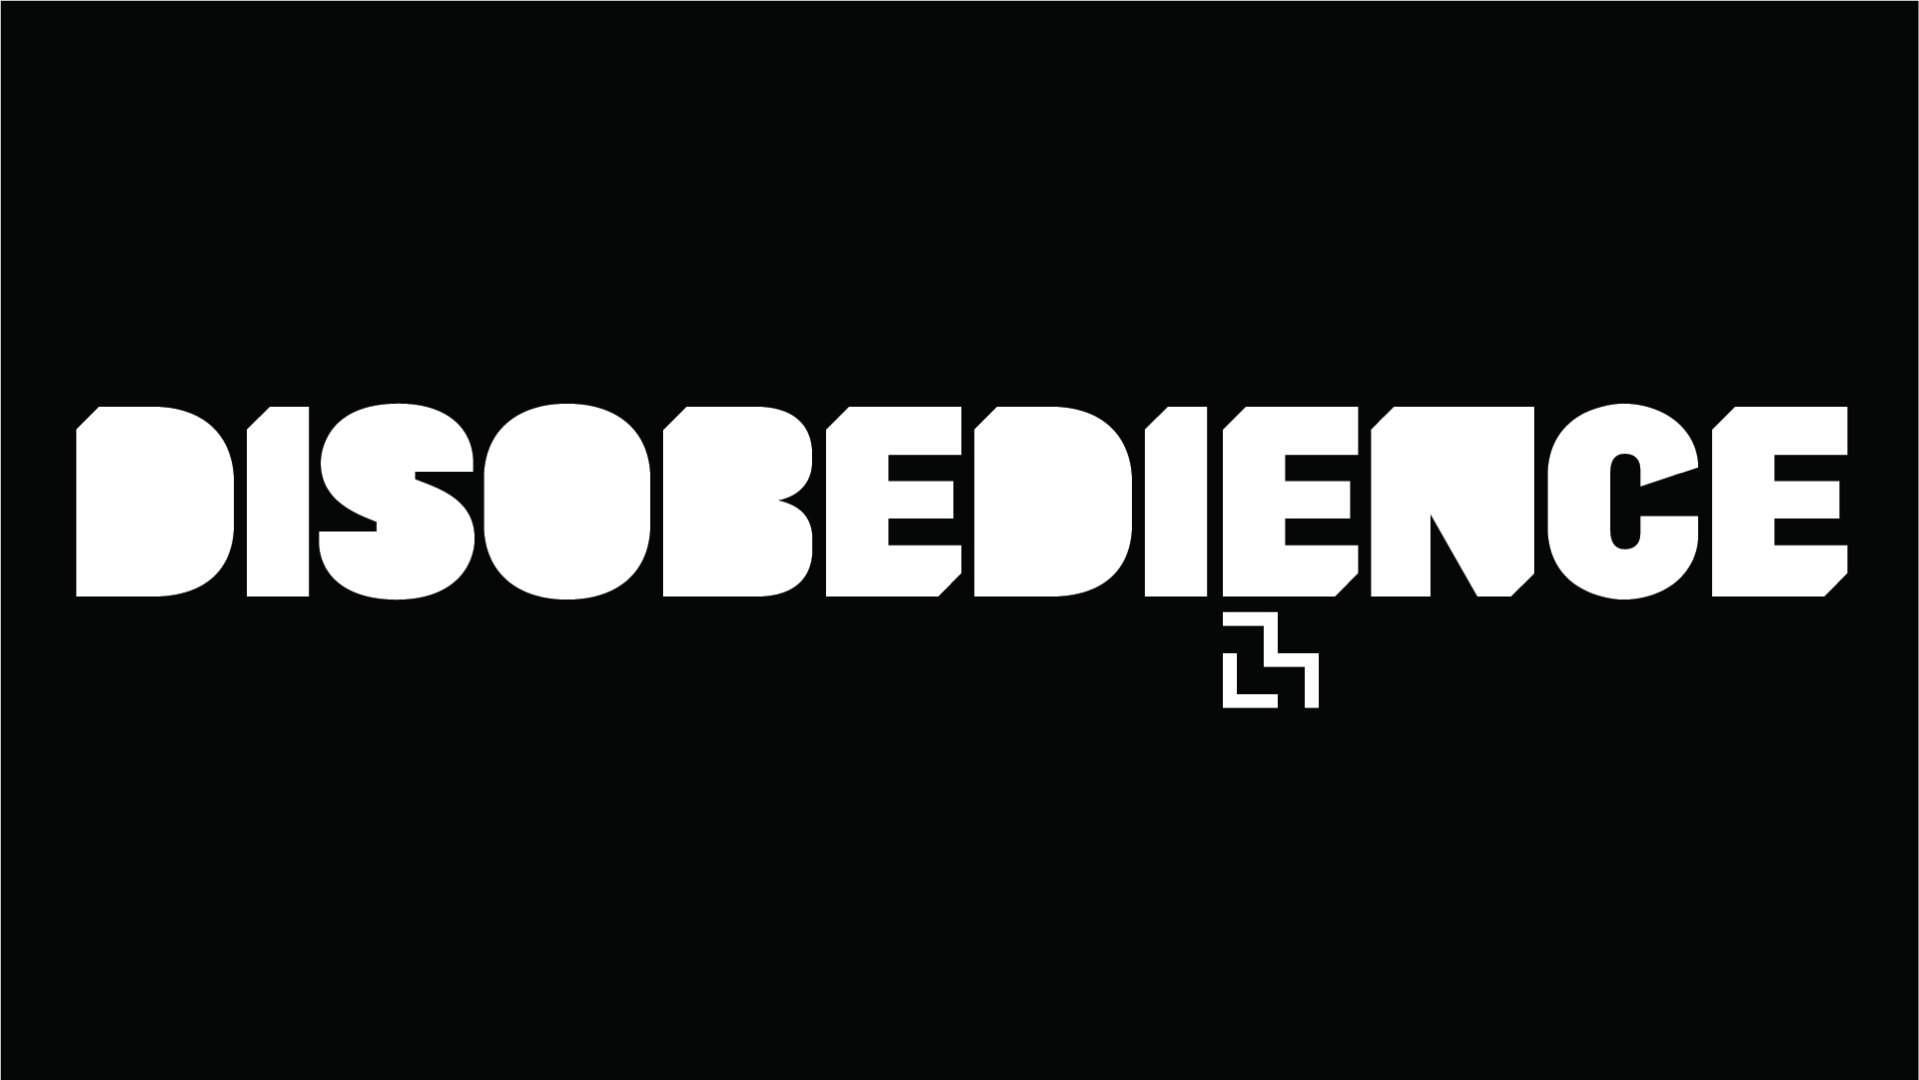
\includegraphics[width=1\textwidth]{pictures/disobedience}
 \caption{A graphic from the award ceremony for the MIT Media Lab Disobedience Award in 2017.}
 \label{fig:disobedience}
\end{figure}

With support of entrepreneur and philanthropist Reid Hoffman, since last year, I have been awarding a \$250,000 prize for disobedience from the Media lab. (Artwork from the prize in \autoref{fig:disobedience}.) As we say on the website \cite{disobedience2018}:

\begin{quote}
This award will go to a person or group engaged in what we believe is an extraordinary example of disobedience for the benefit of society: work that impacts society in positive ways, and is consistent with a set of key principles, including nonviolence, creativity, courage, and responsibility for one’s actions. We invite nominations for work across disciplines (scientific research, civil rights, freedom of speech, human rights, and the freedom to innovate, for example). 
\end{quote}

Last year, we gave the award to Dr. Mona Hanna-Attisha and Professor Marc Edwards. ``Both are scientists who became activists, using rigorous research to investigate the concerns of citizens in Flint, Michigan to unravel a mystery that many in positions of power would have preferred to keep under wraps'' \cite{disobedience2017}.

We believe that this is a small symbolic gesture but sends a signal to our community as well as to the rest of the world that we should support and celebrate positive disobedience.

\section{Civility and Governance}

Although Illich used conviviality to mean ``autonomous and creative intercourse among persons, and the intercourse of persons with their environment,'' it traditionally means friendliness. While one can actually be disobedient in a friendly way (many of my students are), it is easy to be disobedient and disruptive in an unfriendly and uncivil way.

\marginpar{I think that the ultimate role of a leader in a open non-hierarchical system is to tend to its robustness and its resilience --- to focus on its flourishing.}Whether we are talking about trolls on mailing lists as I described in \autoref{sec:emergentdemo} or world leaders taunting the public or other world leaders, the enforcement of civility or conviviality in the more traditional sense appears to be harder in decentralized bottom-up organizations.

In \autoref{intro:design} I wrote about an experiment in the feminist movement that tried to reject the idea of leaders but ended up in an informal and less accountable form of leadership, as described by Jo Freeman in ``The Tyranny of Structurelessness'' \cite{freeman1972tyranny}. Clearly having no structure is not the answer.

One study of guilds in the online game \emph{World of Warcraft} showed that guilds developed roles that focused on managing both the well-being of the players as well as the productivity and success of these guilds \cite{williams2014structural}. For many years, I ran a rather large \emph{World of Warcraft} guild, managing the diverse group of players who were paying money to collaborate with each other; \emph{World of Warcraft} charges a monthly subscription fee. Managing this community was surprisingly similar to to my role as the director of the Media Lab where the primary motivation for participating was not for the money or a very obvious progression path.

Most free and open source projects have similar dynamics --- Wikipedia, Bitcoin, Linux, etc. There is often, but not always, a core group of people who are ultimately in charge. However, most disputes are settled at the local level and through consensus.

Consensus means that everyone reaches an agreement to move forward through discussion. I learned from being on the ICANN board for three years that consensus does not require that everyone ultimately gets what they want, but that you have enough discussion so all voices are heard and the people who object to the majority eventually are convinced or get so tired that they agree to go along. Since everyone was in the room when the decision was made, they can't complain later. At ICANN we would have hours of ``open mic'' where the community would voice objections and grievances, but because we heard them out, we could reach a consensus to move forward.

Consensus doesn't always work. When you can't reach consensus you vote. Voting is never the first choice.

The role of a leader in an open non-hierarchical system is usually to manage the process, sometimes to make tie-breaking decision and sometimes to deal quietly behind-the-scenes with problems that have privacy issues that prevent a public discussion or need a speedy response that a large community can not provide.

However, I think that the ultimate role of a leader in a open non-hierarchical system is to tend to its robustness and its resilience --- to focus on its flourishing. Often it feels like gardening --- watering the plants, sometimes pruning, sometimes moving seedlings, but mostly just making sure that all of the organisms are able to be the best versions of themselves, and creating enough connections and diversity so that the garden is able to fend off the pests and bad weather by itself.

While trolls can always cause trouble as we can see from the polarization in society today, I believe that the best method for dealing with bad culture is good culture. Attacking clostridium difficile with antibiotics doesn't work well but a fecal transplant from a healthy person worked 87 percent of the time in a recent study \cite{jiang2017randomised}. The best way to fight the pathogen is to introduce a diverse and healthy culture, not try to eliminate it. Bombing terrorists has a similar effect to the antibiotics. It kills the healthy culture and makes the negative culture stronger because it ends up with more space, resources and renewed purpose. The old adage, ``Don't feed the trolls'' has a similar point. Getting angry and and focused on the trolls will deplete you of your energy, and is often exactly what the trolls are trying to achieve, giving them more energy and maybe even attracting more.

In``Why Civil Resistance Works,'' Maria J. Stephan and Erica Chenoweth study the strategic effectiveness of violent and nonviolent conflicts between 1900 and 2006. They show that nonviolent campaigns succeeded 53 percent of the time compared to 26 percent of violent resistance campaigns \cite{chenoweth2011civil}. While the success of a nonviolent campaign is still only a coin-toss, it's statistically more likely to succeed in the conflicts that they studied than violent resistance. The notion of ``satyagraha'' or ``truth force,'' espoused by Gandhi \cite{majmudar2012gandhi} is, in my view, the most effective form of non-violent action.

While most non-violent action is typically employed by communities fighting against the establishment, the basic tenets can work in undermining and disabling negative individuals or sub-communities. In the long run ``taking the higher road'' is the most sustainable way to build a a trusting and robust community with a strong positive culture.

\section{Self-Awareness and Humility} 

Whether we are talking about trolls or participant design, the key is to focus on doing a better job yourself instead of trying to tell others what to do or how to do it. I believe that whether we are talking about an individual or an institution, striving for strong core values and excellence, and being open, transparent, and accessible allows others to copy the patterns that work for them in their context. It's important to design organizations for transparency because it's difficult to transform closed organizations into transparent ones \cite{Ito2011Designings}.

Communities are defined by their differences: differences in diversity, size, resources, mission, history, and technical landscapes. Good values can transfer across communities, and adjacent communities can adopt sensibilities and ideas, translating them into local values. We have seen that courage --- from Gandhi's image on the cover of \emph{Life Magazine}, to the Tunisian protesters on social media, to the Parkland students --- can transmit across communities very quickly.

I believe that the most humble, and the most effective, approach to changing the world is to make yourself and your own community better and more flourishing, and to share ideas and connections as freely as possible.

For this, communities and individuals need to become self-aware and reflective so that they --- we --- are able to deprogram the conditioning of decades of institutional education, institutionalized social inequity, and ``greed is good'' justifications for exploitative capitalism. Only thus can we continue to strive to make ourselves better versions of ourselves. 

(How ``better'' is defined will be covered in future work.)
